\documentclass[10pt,twocolumn,letterpaper]{article}

\usepackage{cvpr}
\usepackage{times}
\usepackage{epsfig}
\usepackage{graphicx}
\usepackage{amsmath}
\usepackage{amssymb}
\usepackage{float}
\usepackage{multirow}

% Include other packages here, before hyperref.

% If you comment hyperref and then uncomment it, you should delete
% egpaper.aux before re-running latex.  (Or just hit 'q' on the first latex
% run, let it finish, and you should be clear).
\usepackage[breaklinks=true,bookmarks=false]{hyperref}

\cvprfinalcopy % *** Uncomment this line for the final submission

\def\cvprPaperID{****} % *** Enter the CVPR Paper ID here
\def\httilde{\mbox{\tt\raisebox{-.5ex}{\symbol{126}}}}

% Pages are numbered in submission mode, and unnumbered in camera-ready
%\ifcvprfinal\pagestyle{empty}\fi
\setcounter{page}{1}
\begin{document}

%%%%%%%%% TITLE
\title{EE239AS --- Project Report}

\author{Wilson Chang\\
University of California, Los Angeles\\
{\tt\small ckwojai@ucla.edu}
% For a paper whose authors are all at the same institution,
% omit the following lines up until the closing ``}''.
% Additional authors and addresses can be added with ``\and'',
% just like the second author.
% To save space, use either the email address or home page, not both
\and
Ron Ocampo\\
University of California, Los Angeles\\
{\tt\small ronocampo@ucla.edu}
}

\maketitle
%\thispagestyle{empty}

%%%%%%%%% ABSTRACT
\begin{abstract}
This project explores the use of recurrent neural networks (RNN) for the purpose of classifying electroencephalography (EEG) signals. Results from this project show that convolutional neural networks (CNN) perform more accurately at classifying EEGs compared to the various RNN architectures attempted in this paper. This result is surprising because the structure of RNNs is built around the purpose of analyzing time series information while CNNs are inspired from image processing. 
 
\end{abstract}

%%%%%%%%% BODY TEXT
\section{Introduction}
The architectures implemented in this project were chosen based on increasing levels of complexity. We began testing on the the most simple of RNN and CNN approaches first before attempting more complex hybrids of the two structures. Inspiration for which approach to implement came from current state-of-the-art architectures also used for EEG classification.

In \cite{ChronoNet}, Roy describes ChronoNet, a neural network used for distinguishing between abnormal and normal EEG signals. ChronoNet is motivated as a concatenation of simpler RNN and CNN topologies. Similarly, we began our approach with a basic 3-layer gated recurrent unit (GRU), and assessing its performance before proceeding to a multi-filtered time convolution GRU, named by Roy as Inception Convolutional Gated Recurrent Neural Network (IC-RNN). It was only after attempting these structures that the full ChronoNet architecture was implemented. This paper showed promising results and we were hoping this architecture would yield similar performance for our classification task.

ChronoNet is interesting because it leverages the memory element of RNNs to learn temporal dependencies of the input signal. On the other hand, Schirrmeister in \cite{CNN} uses the convolution operation to capture temporal dependencies. While our focus is on RNN structures, it is worthwhile to investigate the results of \cite{CNN} as a baseline since it uses the same BCI Competition dataset as this project. It was expected that the RNNs would perform better than CNN since their structure is more tailored for varying time series data.

\section{Results}
The dataset are divided into training, validation, and testing datasets and are trained on all our models. For subject 1 dataset, training data are mini-batched 50 datapoints per batch and there are 50 datapoints for both validation and testing datasets. For all subject dataset, training data are mini-batched 200 datapoints per batch and there are 100 datapoints for both validation and testing datasets. We then trained our model for 10 epochs and report the best validation accuracy. \par

In reference to Table \ref{tab:algo}, we record the validation accuracy and put it in a table. Results suggest that models trained on all subjects yield a better validation accuracy versus only on subject 1. With the highest positive gain of 10\% for Shallow CONV model, and around 2-5\% increase for RNN models. \par

We also observed that a bigger dataset highly eases the pitfall of overfitting of RNN architectures, with training accuracies reaching over 90 \% for most RNNs trained on only subject 1 data. Meanwhile, for models trained in all subjects, training accuracies are around 60-70 \% when the models reaches its best validation accuracy. \par

In reference to Figure \ref{fig:lstm_acc} and \ref{fig:gru_acc}, we test how our RNN model behaves on the simple LSTM and GRU models as we train the network with increasing time sequence of data from 0 to 1000 with increment of 100. Surprisingly, both the LSTM and GRU models show a drastic decrease of performance as we feed the RNN model longer time sequence data. \par


Hidden size of the RNN models are specifically tuned to avoid overfitting and maximize validation accuracy. For subject 1 data, any hidden size over 10 strongly overfits the data, reaching more than 90 \% training accuracy within 10 epochs. For all subjects data, since we have more data, we increase the hidden size to 32 to better fit the data and optimize validation accuracy. In addition, it also make convenient for the convolution layers. \par

To compare the accuracies among models, a simple 1-layer LSTM with 32 hidden units outperforms all other stacked layer of pure RNN structures, namely a 3-Layer-LSTM with dropout which expects to have a regularization effect and the 3-layer-GRU. We argue that adding more layers to RNN doesn't help the classification task because it led to strong overfitting. A similar argument was also made in by Juri Fedjaev in his master thesis \cite{LSTM}, that a 1 layer LSTM works better than deeper model for EEG data. \par

All in all, we tried a lots of different RNN architectures, including LSTM and GRU and their variance such as adding Convolutional layers before RNN layers. However, suffering from overfitting, validation accuracies fluctuate between 20 - 40 \% for all these architectures. In particular, ChronoNet \cite{ChronoNet}, which has specially designed concatenated convolution layer, scores the best validation accuracy 40 \% among all the RNN architectures. However, the performance is still not as ideal as a pure CNN, which scores a incredibly 72\% validation accuracy.
 
\section{Discussion}
In the results outlined in the previous section, the raw EEG data was feed directly as input the to neural network. The intuition behind this is that a properly trained network would be able to learn the relevant features for classification all on its own.  This mentality, however, could have been the crux as to why the RNNs in this project did not perform as well as CNN in the Shallow CONV architecture. 

The input to the RNN is time in one dimension and the respective electrode in another dimension. The memory aspect of RNNs learn relevant dependencies in time, but largely only within their respective electrode. The two dimensional convolution and pooling layer of Shallow CONV allows the this network to learn temporal as well as spatial dependencies. The lack of the spatial aspect could be a key reason as to why RNNs were not performing as well. The ChronoNet architecture could be misleading since it does incorporate different sized convolution filters concatenated together. These convolutions, however, are only performed across one dimension, time. Roy mentions "convert[ing] the recorded EEG signal into a set of montages"\cite{ChronoNet}. Preprocessing the data in this matter rather than feeding in the raw EEG channels could be the missing piece to achieving meaningful results with RNNs.

This importance of spatial dependence between electrodes can be supported by the fact that EEGs have been believed to have low spatial resolution. As a result, multiple electrodes, spatially, are required to read the relevant EEG signal. When we are analyzing one electrode at a time with our RNN structures, the EEG signal could likely be contaminated with noise. This can be why recent research has implemented spatial filters for increasing signal-to-noise ratio of EEG signals for brain-computer interfaces \cite{DBLP:journals/corr/WuKCLJ17}.

In this paper only temporal preprocessing was attempted and not spatially. One such technique was to use the time derivative of the EEG signal. The inspiration from this approach came from the use of first and second derivatives for spike sorting of electromyography (EMG) signals \cite{EMG}. The intuition is that EEG signals when a subject this thinking of moving his or her hands versus feet, for example, may spike at different rates. To feed this information into the network, this feature vector was concatenated to the 23 electrodes yielding a (46,1000) input matrix for each training example.

Another preprocessing technique we tried to implement was form of data augmentation. During the length one 1000 sample trial the subject is instructed the same thing.  This one trial could then be split into multiple smaller trails, be given the same label as the original trial and be feed into the network as a new training example. We split each trail into ten 100 sample long segments. When training with all 10 subjects, this technique increased the training set by 100 times. Talathi \cite{Deep} used this approach for their seizure detection GRU based network. The potential benefit of this is twofold. Neural networks benefit from more data and reducing the time dimension facilities training. RNN structures have a lot of parameters and become computational bottleneck in these networks. A lower time dimension speeds up the RNN layers.

Overall both of these preprocessing techniques did not help to make our RNNs perform even as well Shallow CONV. The reason for this goes back to the argument of spatial information and learning. Both of these techniques only operated on the temporal dimension of the signal. For future work, we would interested in revisiting the ChronoNet architecture but with implementing a two dimensional convolution such as Shallow CONV. RNN structures did not show to perform better than CNN in this paper, but we feel that they can still have value in EEG signal classification if care is taken to ensure spatial learning is also incorporated into the network.
\clearpage
\newpage
{\small
\bibliographystyle{ieee}
\bibliography{egbib}
}

%% ============================================================
%% Two Extra Pages
%% ============================================================
 \clearpage
\newpage
\clearpage
\newpage
\clearpage
\newpage
\section{Algorithm and Performance}
\begin{table}[h]
  \centering
  \begin{tabular}{lccc}
    \hline
    Model & Hidden Size & Subject 1 & All subjects\\
    \hline
    1 layer LSTM & 10/32 & 0.35 & 0.38\\
    3 layer LSTM, DO & 64/32 & 0.28 & 0.30\\
    Incept-LSTM & 10/32 & 0.30 & 0.35\\
    GRU & 10/32 & 0.32 & 0.34\\
    Incept-GRU & 10/32 & 0.31 & 0.35 \\
    ChronoNet & 10/64 & 0.4 & 0.4\\
    Shallow CONV & 32/32 & 0.62 & 0.72\\
    \hline
  \end{tabular}
  \caption{Table of Algorithm Performance}\label{tab:algo}
\end{table}

\begin{figure}[h]
  \centering
  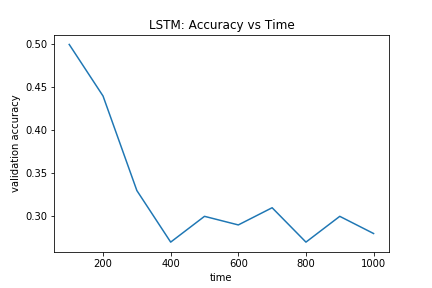
\includegraphics[scale=0.5]{t_LSTM}
  \caption{LSTM: accuracy vs time}
  \label{fig:lstm_acc}
\end{figure}

\begin{figure}[h]
  \centering
  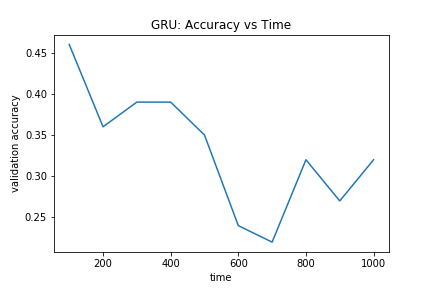
\includegraphics[scale=0.5]{t_GRU}
  \caption{GRU: accuracy vs time}
  \label{fig:gru_acc}
\end{figure}
\newpage
\section{Architectures}
\begin{table}[h]
  \centering
  \begin{tabular}{l|l}
    Model & Description\\
    \hline
    1 layer LSTM & LSTM\\
    3 layer LSTM, DO & (LSTM-DO)x3 \\
    Incept-LSTM & Inception-LSTM-LSTM-LSTM\\
    GRU & GRU\\
    Incept-GRU & Inception-GRU-GRU-GRU\\
    ChronoNet & Inceptx3-GRUx3\\
    Shallow Conv & Convx2-MeanPool\\    
  \end{tabular}
  \caption{Table of Architectures}
\end{table}

\textbf{LSTM / GRU} \\
A one layer LSTM/GRU has structure similar to the following \\
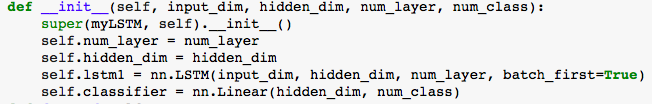
\includegraphics[scale=0.4]{stru_LSTM} \\ \\
\textbf{LSTMx3} \\
A three layer LSTM has structure as shown below \\
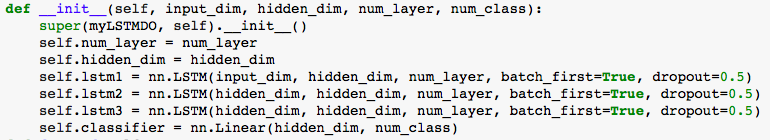
\includegraphics[scale=0.35]{stru_LSTMDO} \\ \\
\textbf{Inception-LSTM/GRU} \\
The motivation of adding a inception layer before LSTM/GRU is the filtering nature of inception layer. The ability of convolution layers to extract features act like a preprocessor of the raw EEG data. With this in mind, we borrow the inception layer structure from a CNN paper \cite{CNN}. Instead of filter number of 40 in the second stacked convolution, we make the filter number 23 in order to match the number of electrode. \par
The Pytorch implementation is shown below. \\
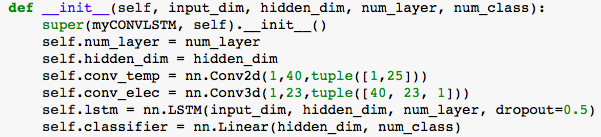
\includegraphics[scale=0.45]{stru_CONVLSTM} \\ \\
\textbf{ChronoNet} \\
ChronoNet is an architecture specifically design to extract features from EEG data. Multiple filters with exponential size is implemented in each Conv1D layer (total of three). This allows extracting features spanning over multiple time scale. \par
Moreover, over the very last 3 stacks of GRU layers, skip connection is implemented to deal with degradation. This allows GRU layers to ignore GRU outputs when model complexity is low on the entire network. \cite{ChronoNet} \\
The Pytorch implementation is shown below. \\
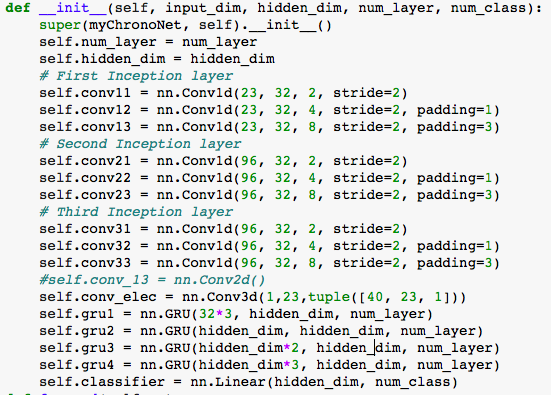
\includegraphics[scale=0.45]{stru_ChronoNet} \\ \\
\textbf{Shallow Convolution} \\
This is the Shallow CNN architecture we borrow from the paper ```Convolutional neural networks in EEG analysis''. We choose this because the validation accuracy is not that far off from the Deep CNN and it's simpler to implement. A temporal convolution layer followed by a spatial convolution layer is done because implicitly defining these layer has a regularization effect on the overall convolution. A mean pooling layer then followed. \cite{CNN} \\ 
The Pytorch implementation is shown below, NOTE that the filter size is modified to retain convolution size for our data \\
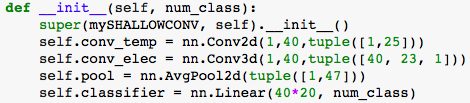
\includegraphics[scale=0.5]{stru_SHALLOW} \\ \\
\end{document}



